\documentclass[hyperref={hidelinks}]{beamer}

\setbeamertemplate{bibliography item}{\insertbiblabel}

\mode<presentation>
\usetheme{Frankfurt}
\usecolortheme{seahorse}

\usepackage{physics}
\usepackage{multimedia}
\usepackage{graphicx}
\usepackage{subcaption}
\usepackage{siunitx}
\usepackage{amsmath}
\usepackage{amssymb}
\usepackage[style=numeric-comp,backend=biber]{biblatex}
\usepackage{cleveref}
\usepackage{tikz}

\usetikzlibrary{patterns}

\addbibresource{biblio.bib}

\usefonttheme[onlymath]{serif}

%% For the Hindmarsh-Rose model
\newcommand*{\hrx}{x}
\newcommand*{\hry}{y}
\newcommand*{\hrz}{z}
\newcommand*{\hra}{\alpha}
\newcommand*{\hrb}{\beta}

%% For the chimera-like index
\newcommand*{\chimera}{\chi}
\newcommand*{\meta}{m}
\newcommand*{\ordparam}{r}
\newcommand*{\phase}{\phi}

%% To make the bibliography fit on one slide
\renewcommand*{\bibfont}{\tiny}

\author{Henry Mitchell \inst{1,2,5} \and
  Peter Dodds \inst{1,4,5} \and
  Matt Mahoney \inst{3,4} \and
  Chris Danforth \inst{1,4,5}
}

\institute{
  \inst{1} UVM Department of Mathematics and Statistics
  \inst{2} UVM Department of Physics \\
  \inst{3} UVM Department of Neurology
  \inst{4} UVM Department of Computer Science \\
  \inst{5} Computational Story Lab
}

\titlegraphic{
\includegraphics[width=2cm]{figure/roboctopus}\hspace*{4.75cm}~%
  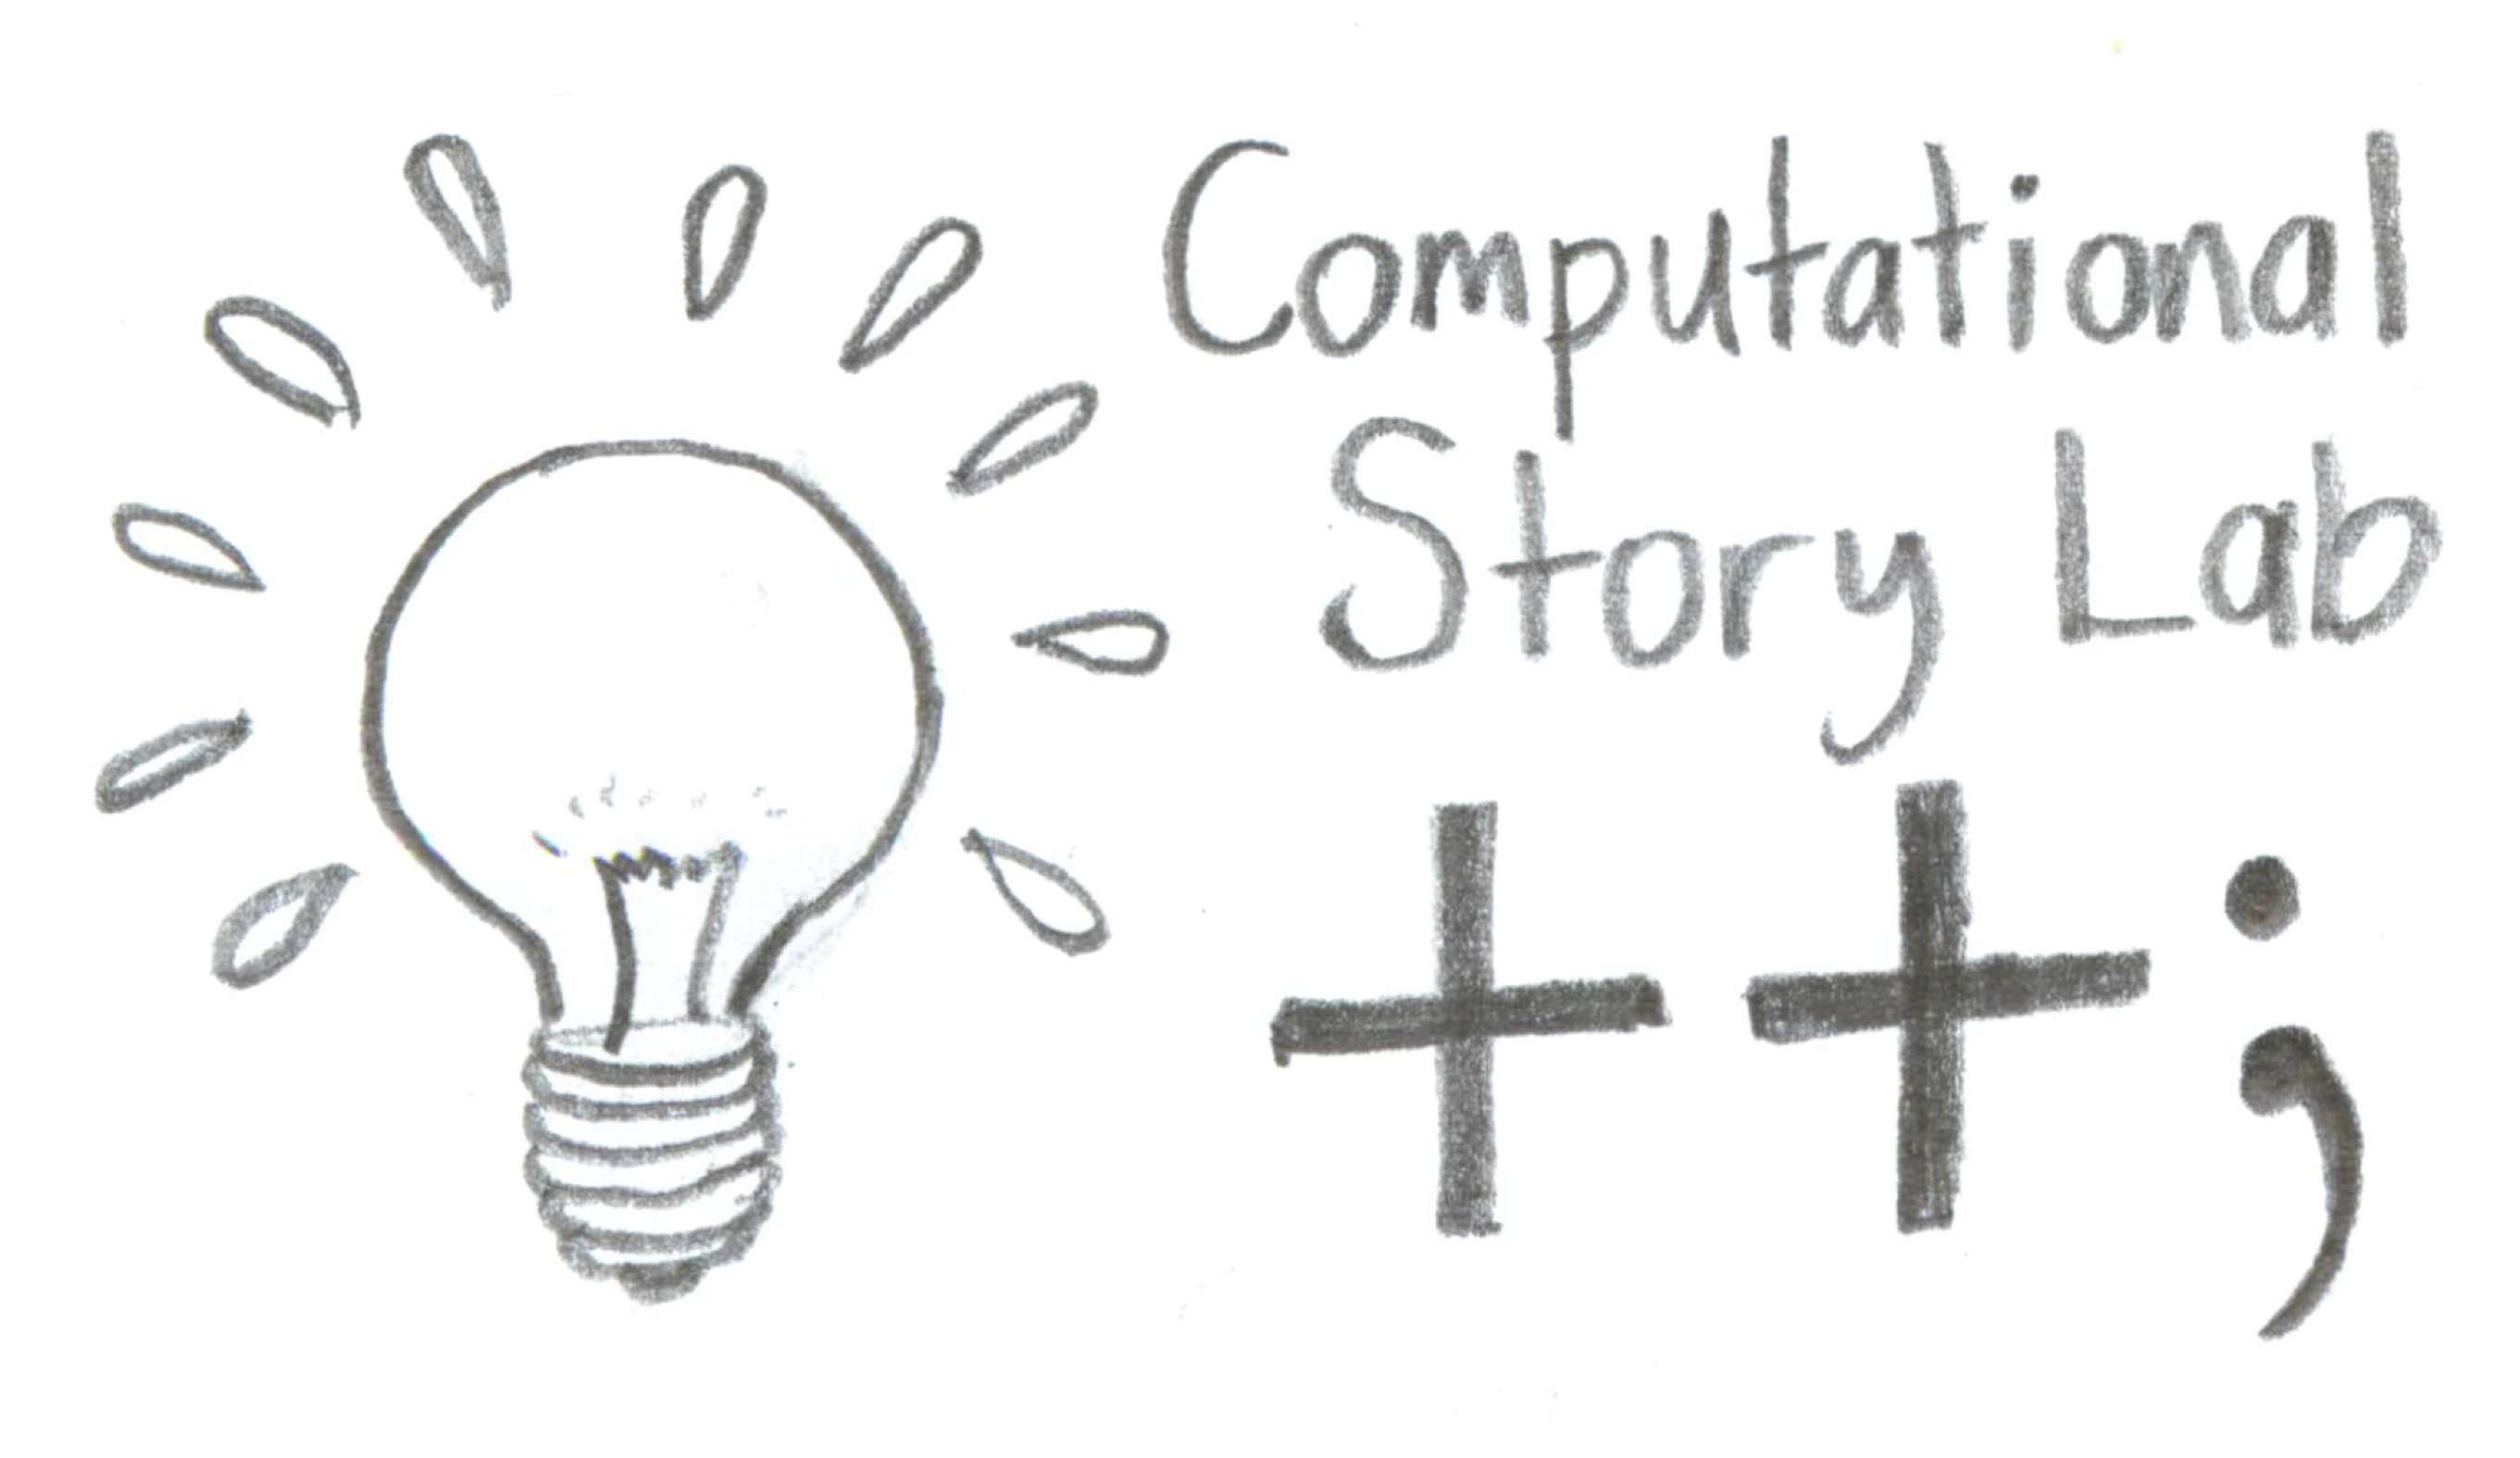
\includegraphics[width=2cm]{figure/storylab}
}

\title{Chimera States and Seizures in a Mouse Neuronal Model}

\begin{document}

\frame{\titlepage}


\section{Chimera states\ldots}
\begin{frame}
  \frametitle{Chimera States}
  A chimera state is \textbf{the coexistence of synchronous and asynchronous populations in a network of nonlocally-coupled oscillators} \cite{Abrams2004,Kuramoto2002}.
  \vfill

  \movie[width=\textwidth,height=0.18\textwidth,autostart,loop=1]{A mechanical example of a chimera state}{figure/mechanical_chimera.mov}
\end{frame}

\begin{frame}
  \frametitle{Measures}
The \textbf{chimera-like index} $\chimera$ is a useful measure for how chimeric a system is.
  \begin{equation}
    \chimera
    =
      \expval{\sigma_{\text{chi}}}_{T}
    \text{ where}\quad
      \sigma_{\text{chi}}(t)
    =
      \frac{1}{M - 1} \sum_{c \in C}\pqty{\ordparam_{c}(t) - \expval{\ordparam_{c}}_{C}}^{2}
    \label{eq:chimera}
  \end{equation}
  and $\ordparam_{c}$ is the order parameter of community $c$.
  It is the \textbf{time average of the variance between communities of the order parameter}.
  Its maximum value is $1/7$, and will be normalized as such.

\end{frame}

\section{\ldots And Seizures\ldots}
\begin{frame}
  \frametitle{Seizures}
  Seizures are \textbf{excessive(ly) synchronous neural activity} \cite{Kandel2013}.
  Focal seizures occur when parts of the brain seize while the rest behaves normally.
  \begin{figure}[ht]
    \centering
    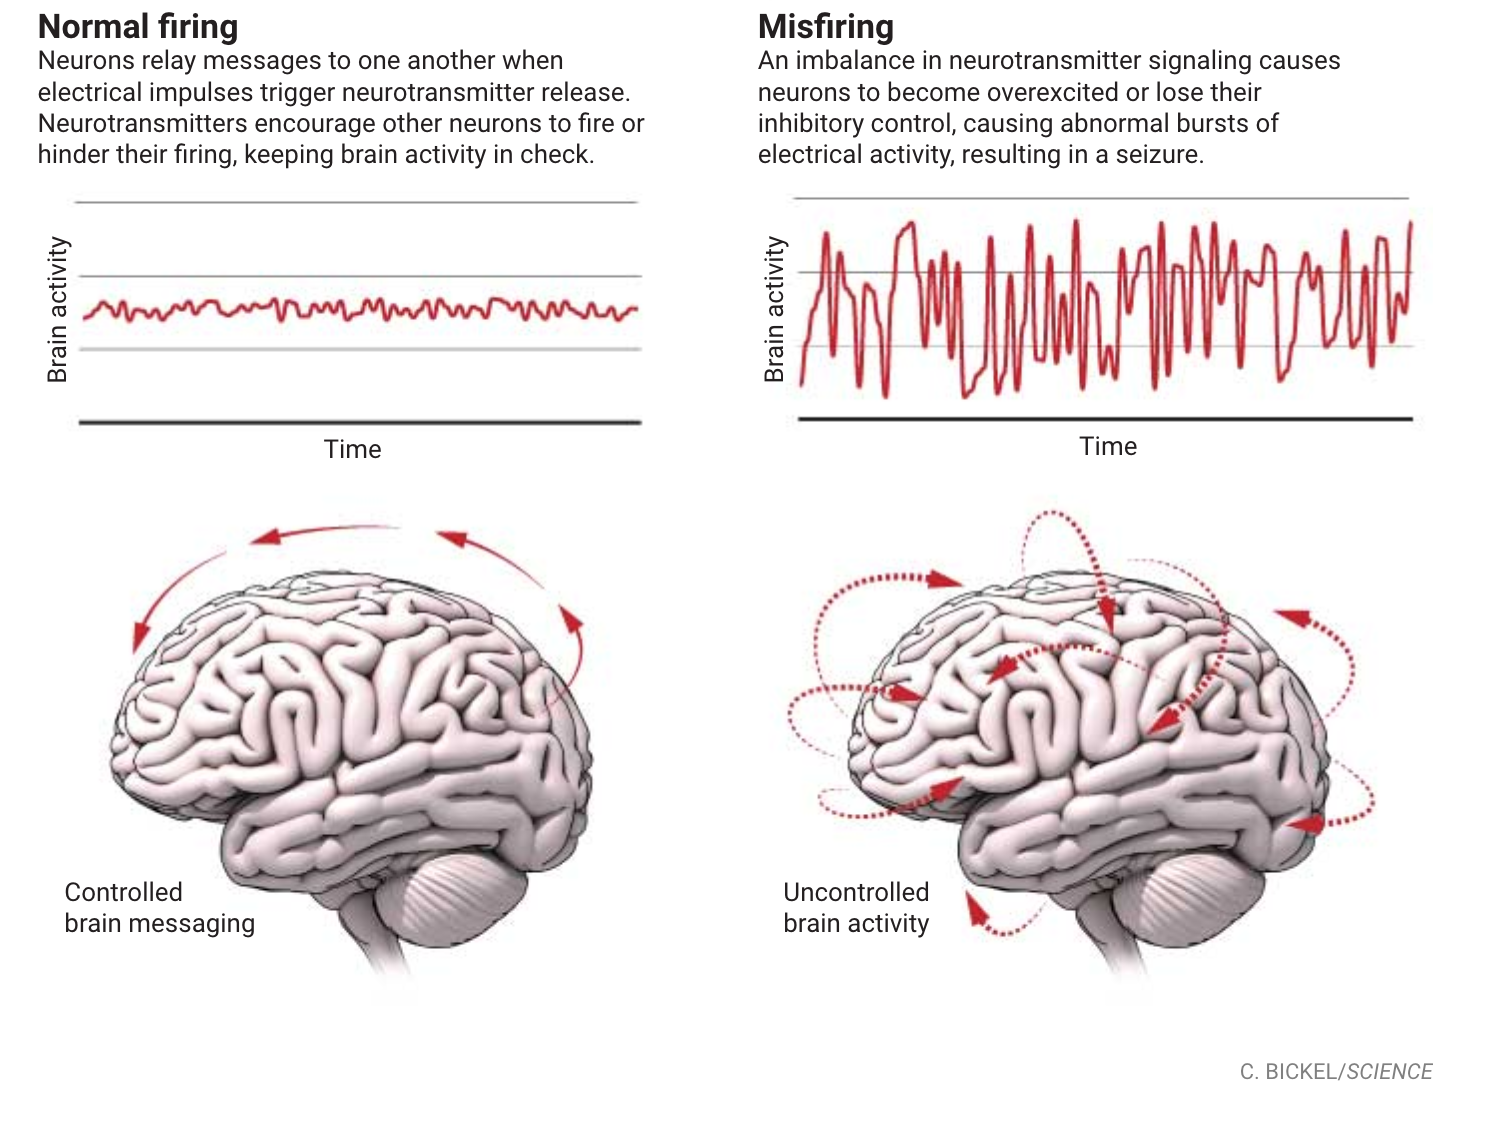
\includegraphics[width=0.75\textwidth]{figure/seizure}
  \end{figure}

\end{frame}


\section{\ldots In a Mouse Neuronal Model}
\begin{frame}
  \frametitle{The Mouse Connectome}
  The oscillator network was modeled after the mouse connectome \cite{Oh2014}.
  \begin{figure}
    \centering
    \begin{subfigure}{0.49\textwidth}
      \centering
      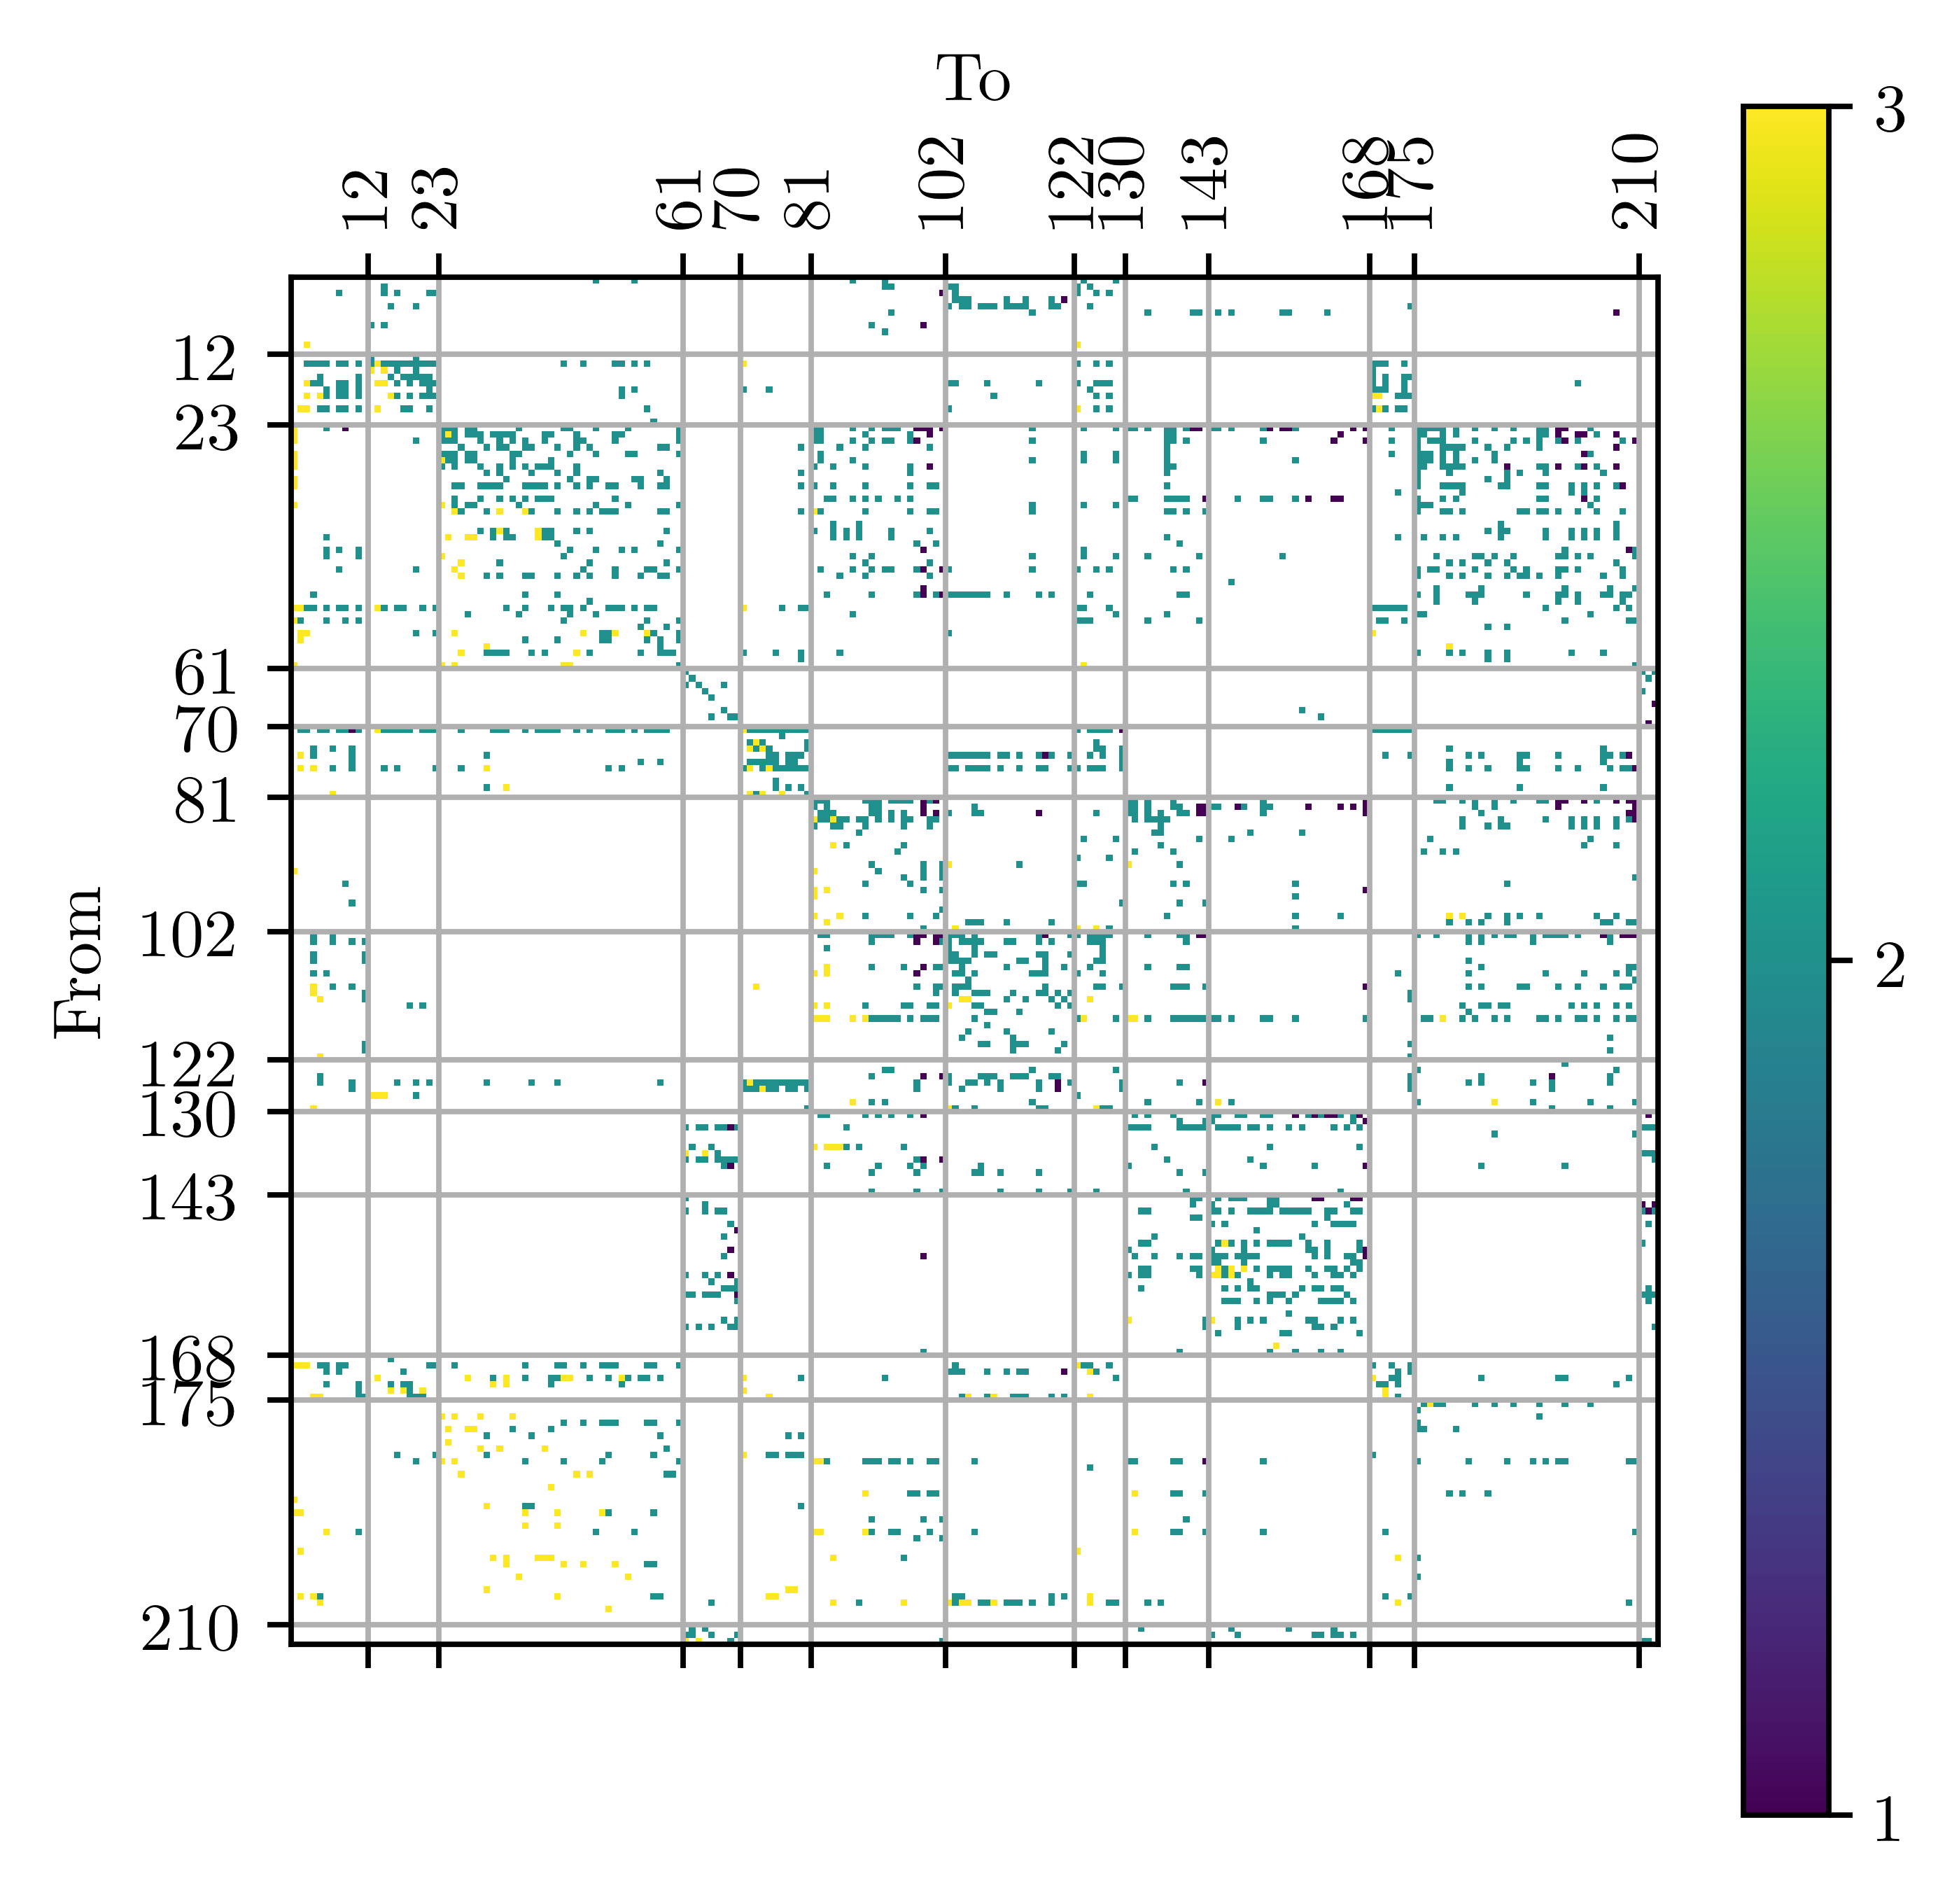
\includegraphics[width=0.99\textwidth]{figure/n}
      \caption{}
      \label{fig:connectome_matrix}
    \end{subfigure}%
    \begin{subfigure}{0.49\textwidth}
      \centering
      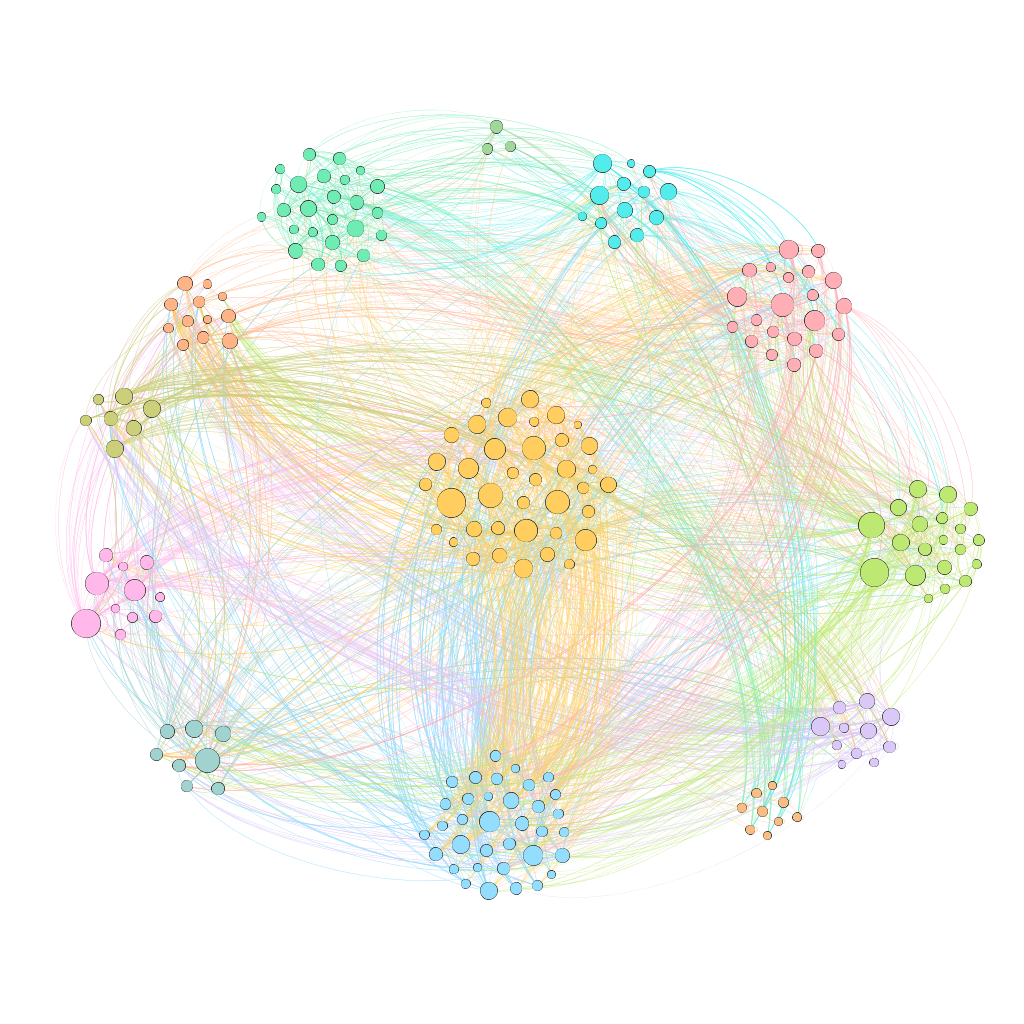
\includegraphics[width=0.99\textwidth]{figure/network}
      \caption{}
      \label{fig:connectome_embedding}
    \end{subfigure}
    \label{fig:connectome}
  \end{figure}

\end{frame}

\begin{frame}
  \frametitle{Model Parameters}
  \begin{table}[ht]
    \centering
    {\tiny
      \begin{tabular}{c | c | l}
        Symbol & Value & Meaning \\ \hline
        $\hrx_{j}$ & --- & \textbf{Membrane potential of the $j$th neural mass} \\
        $\hry_{j}$ & --- & \textbf{Associated with fast intra-neural processes} \\
        $\hrz_{j}$ & --- & \textbf{Associated with slow intra-neural processes} \\ \hline
        $b$ & 3.2 & Tunes the spiking frequency \\
        $I_{j}$ & 4.4 & External input current \\
        $\hrx_{\text{rev}}$ & 2 & Ambient reverse potential \\
        $\lambda$ & 10 & Sigmoidal activation function parameter \\
        $\theta$ & -0.25 & Sigmoidal activation function parameter \\
        $\mu$ & 0.01 & Time scale for variation of $z$ \\
        $s$ & 4 & Governs adaptation \\
        $\hrx_{\text{rest}}$ & -1.6 & Resting/equilibrium potential \\ \hline
        $\hra$ & Varied & \textbf{Connection strength within cortices} \\
        $n_{j}'$ & \Cref{fig:connectome_matrix} & \textbf{Number of connections within a cortex from the $j$th neuron} \\
        $G'$ & \Cref{fig:connectome_matrix} & \textbf{Intra-cortical connection matrix} \\
        $\hrb$ & Varied & \textbf{Connection strength between cortices} \\
        $n_{j}''$ & \Cref{fig:connectome_matrix} & \textbf{Number of connections between cortices from the $j$th neuron} \\
        $G''$ & \Cref{fig:connectome_matrix} & \textbf{Inter-cortical connection matrix}
      \end{tabular}
      \caption[Hindmarsh-Rose Parameters]{The list of parameters used in modeling the Hindmarsh-Rose network.}
      \label{tab:hr_params}
    }
  \end{table}
\end{frame}

\begin{frame}
  \frametitle{The Model}
  We used a network of modified Hindmarsh-Rose neurons \cite{Santos2017}:
  \begin{align}
    \label{eq:hr_x}
    \begin{split}
      \dot{\hrx}_{j}
      ={}&
      \hry_{j}
      -
      \hrx_{j}^{3}
      +
      b \hrx_{j}^{2}
      +
      I_{j}
      -
      \hrz_{j} \\
      &\quad -
      \frac{\hra}{n'_{j}} \sum_{k ={} 1}^{N} G'_{j k} \Theta_{j}(\hrx_{k})
      -
      \frac{\hrb}{n''_{j}} \sum_{k ={} 1}^{N} G''_{j k} \Theta_{j}(\hrx_{k})
    \end{split} \\
    \label{eq:hr_y}
    \dot{\hry}_{j}
    ={}&
         1
         -
         5 \hrx_{j}^{2}
         -
         \hry_{j} \\
    \label{eq:hr_z}
    \dot{\hrz}_{j}
    ={}&
         \mu \pqty{s \bqty{\hrx_{j} - \hrx_{\text{rest}}} - \hrz_{j}}
  \end{align}
  where
  \begin{equation}
    \label{eq:hr_sigmoid}
    \Theta_{j}(\hrx_{k})
    =
    \frac{\hrx_{j} - \hrx_{\text{rev}}}{1 + e^{-\lambda \pqty{\hrx_{k} - \theta}}}
  \end{equation}
  This sigmoidal activation function helps make the model apply to groups of neurons (subcortices) instead of single neurons.

\end{frame}

\section{Results}
\begin{frame}
  \frametitle{Simulated EEG Output}
  \begin{figure}[ht]
    \centering
    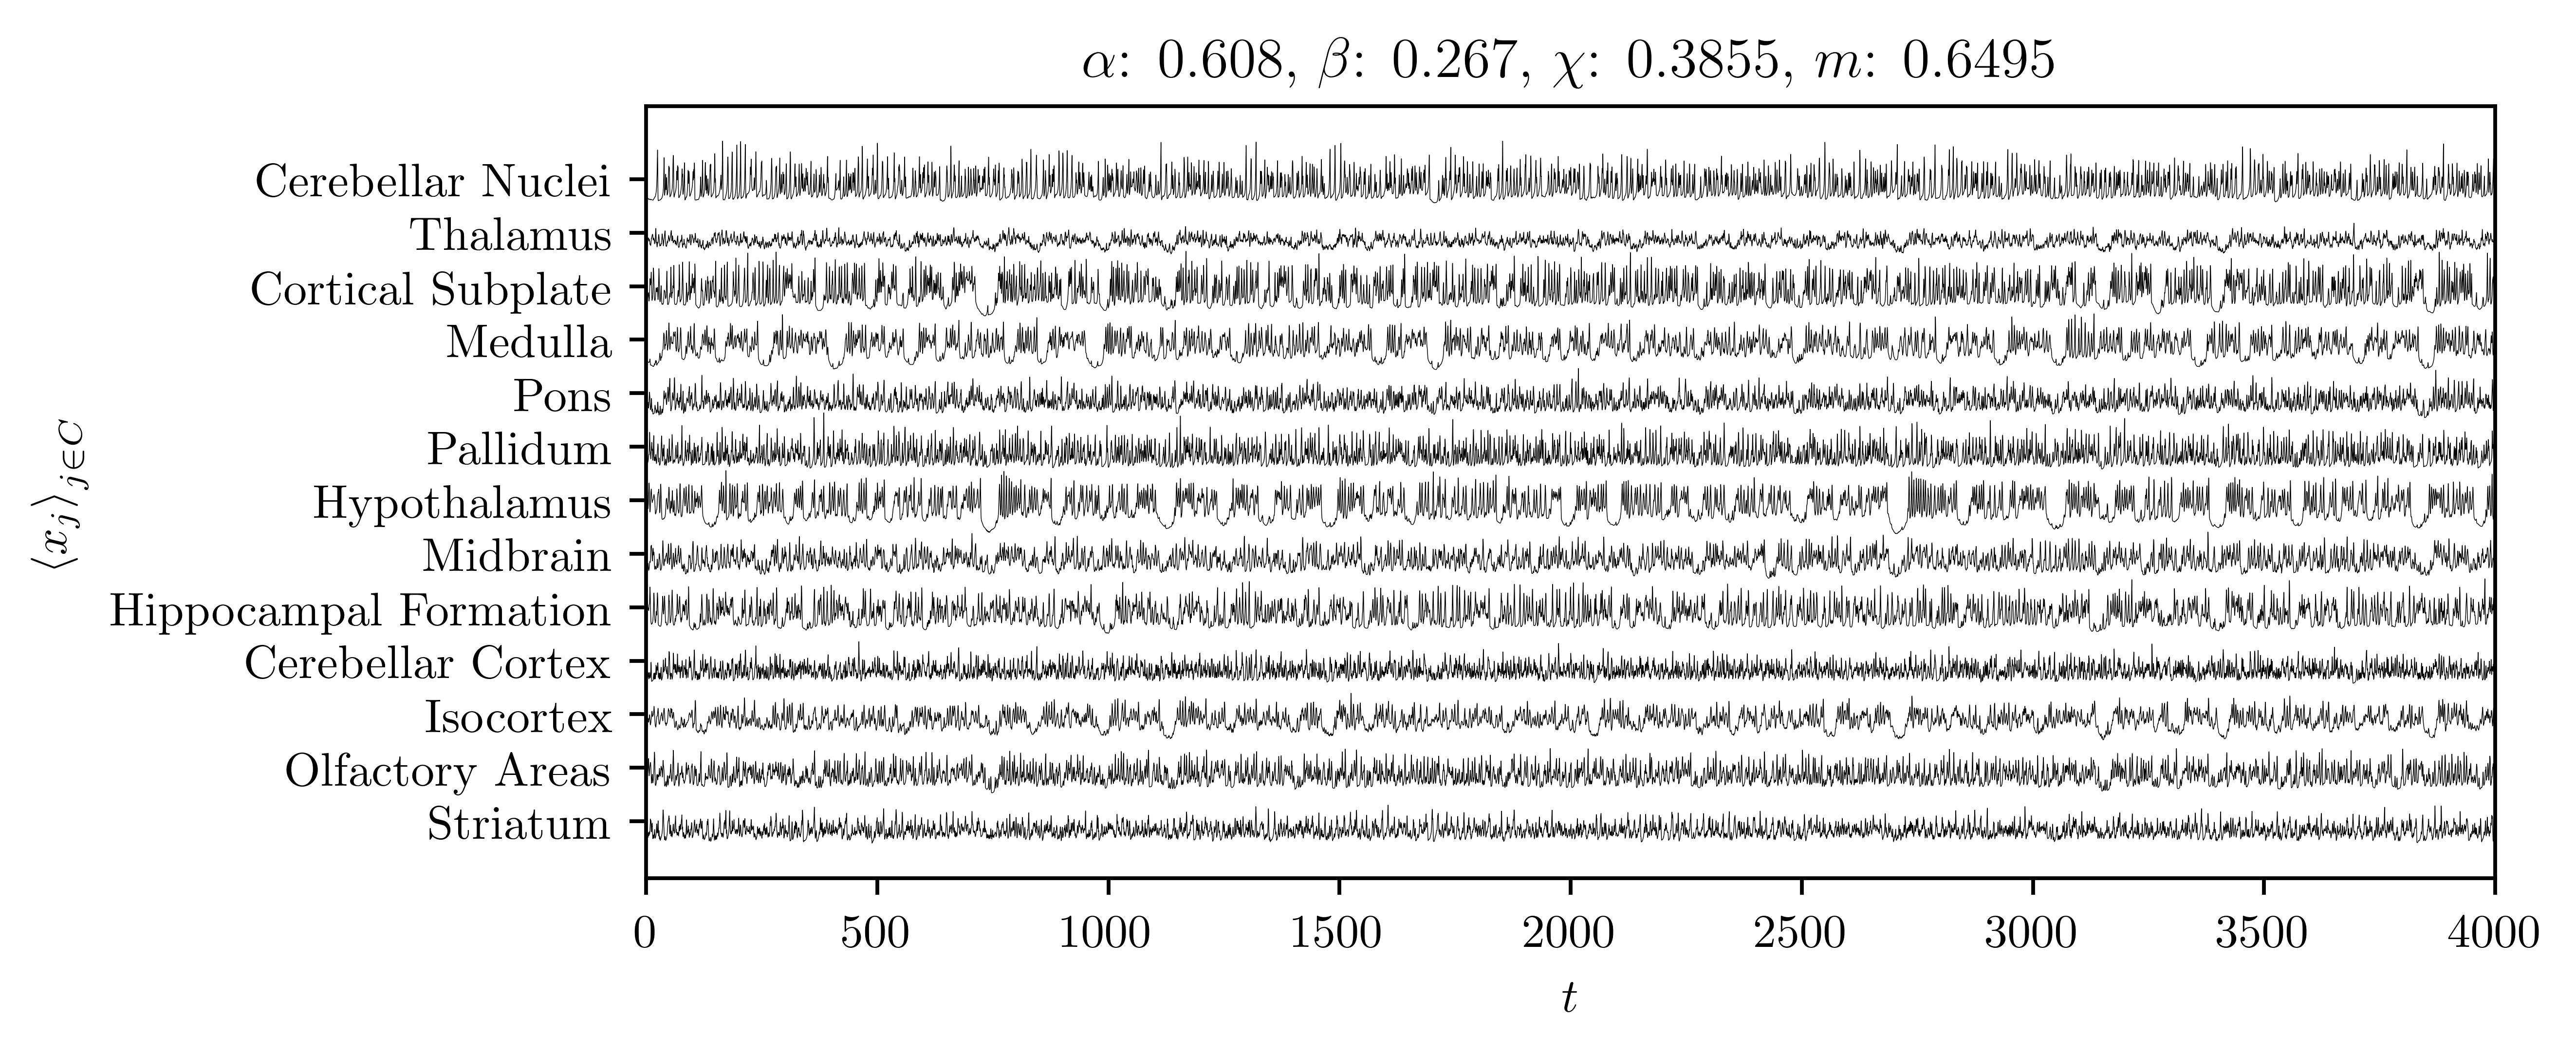
\includegraphics[width=0.95\textwidth]{figure/means-0_608-0_267}
    \caption[Mean potential by cortex]{The mean membrane potential within each cortex.
    }
    \label{fig:mean_608_267}
  \end{figure}
  Thalamus, Pons, Striatum --- wild type

  Cerebellar cortex --- spiking behavior, spike runs

  Medulla, Hypothalamus --- repetitive spike runs

  Cortical subplate --- seizure-like behavior

\end{frame}

\begin{frame}
  \frametitle{Model Physicality}
  The neurons only collectively fired for certain values of $\hra$ (intra-cortical coupling) and $\hrb$ (inter-cortical coupling) \cite{Mitchell2019}.
  \begin{figure}[ht]
    \centering
    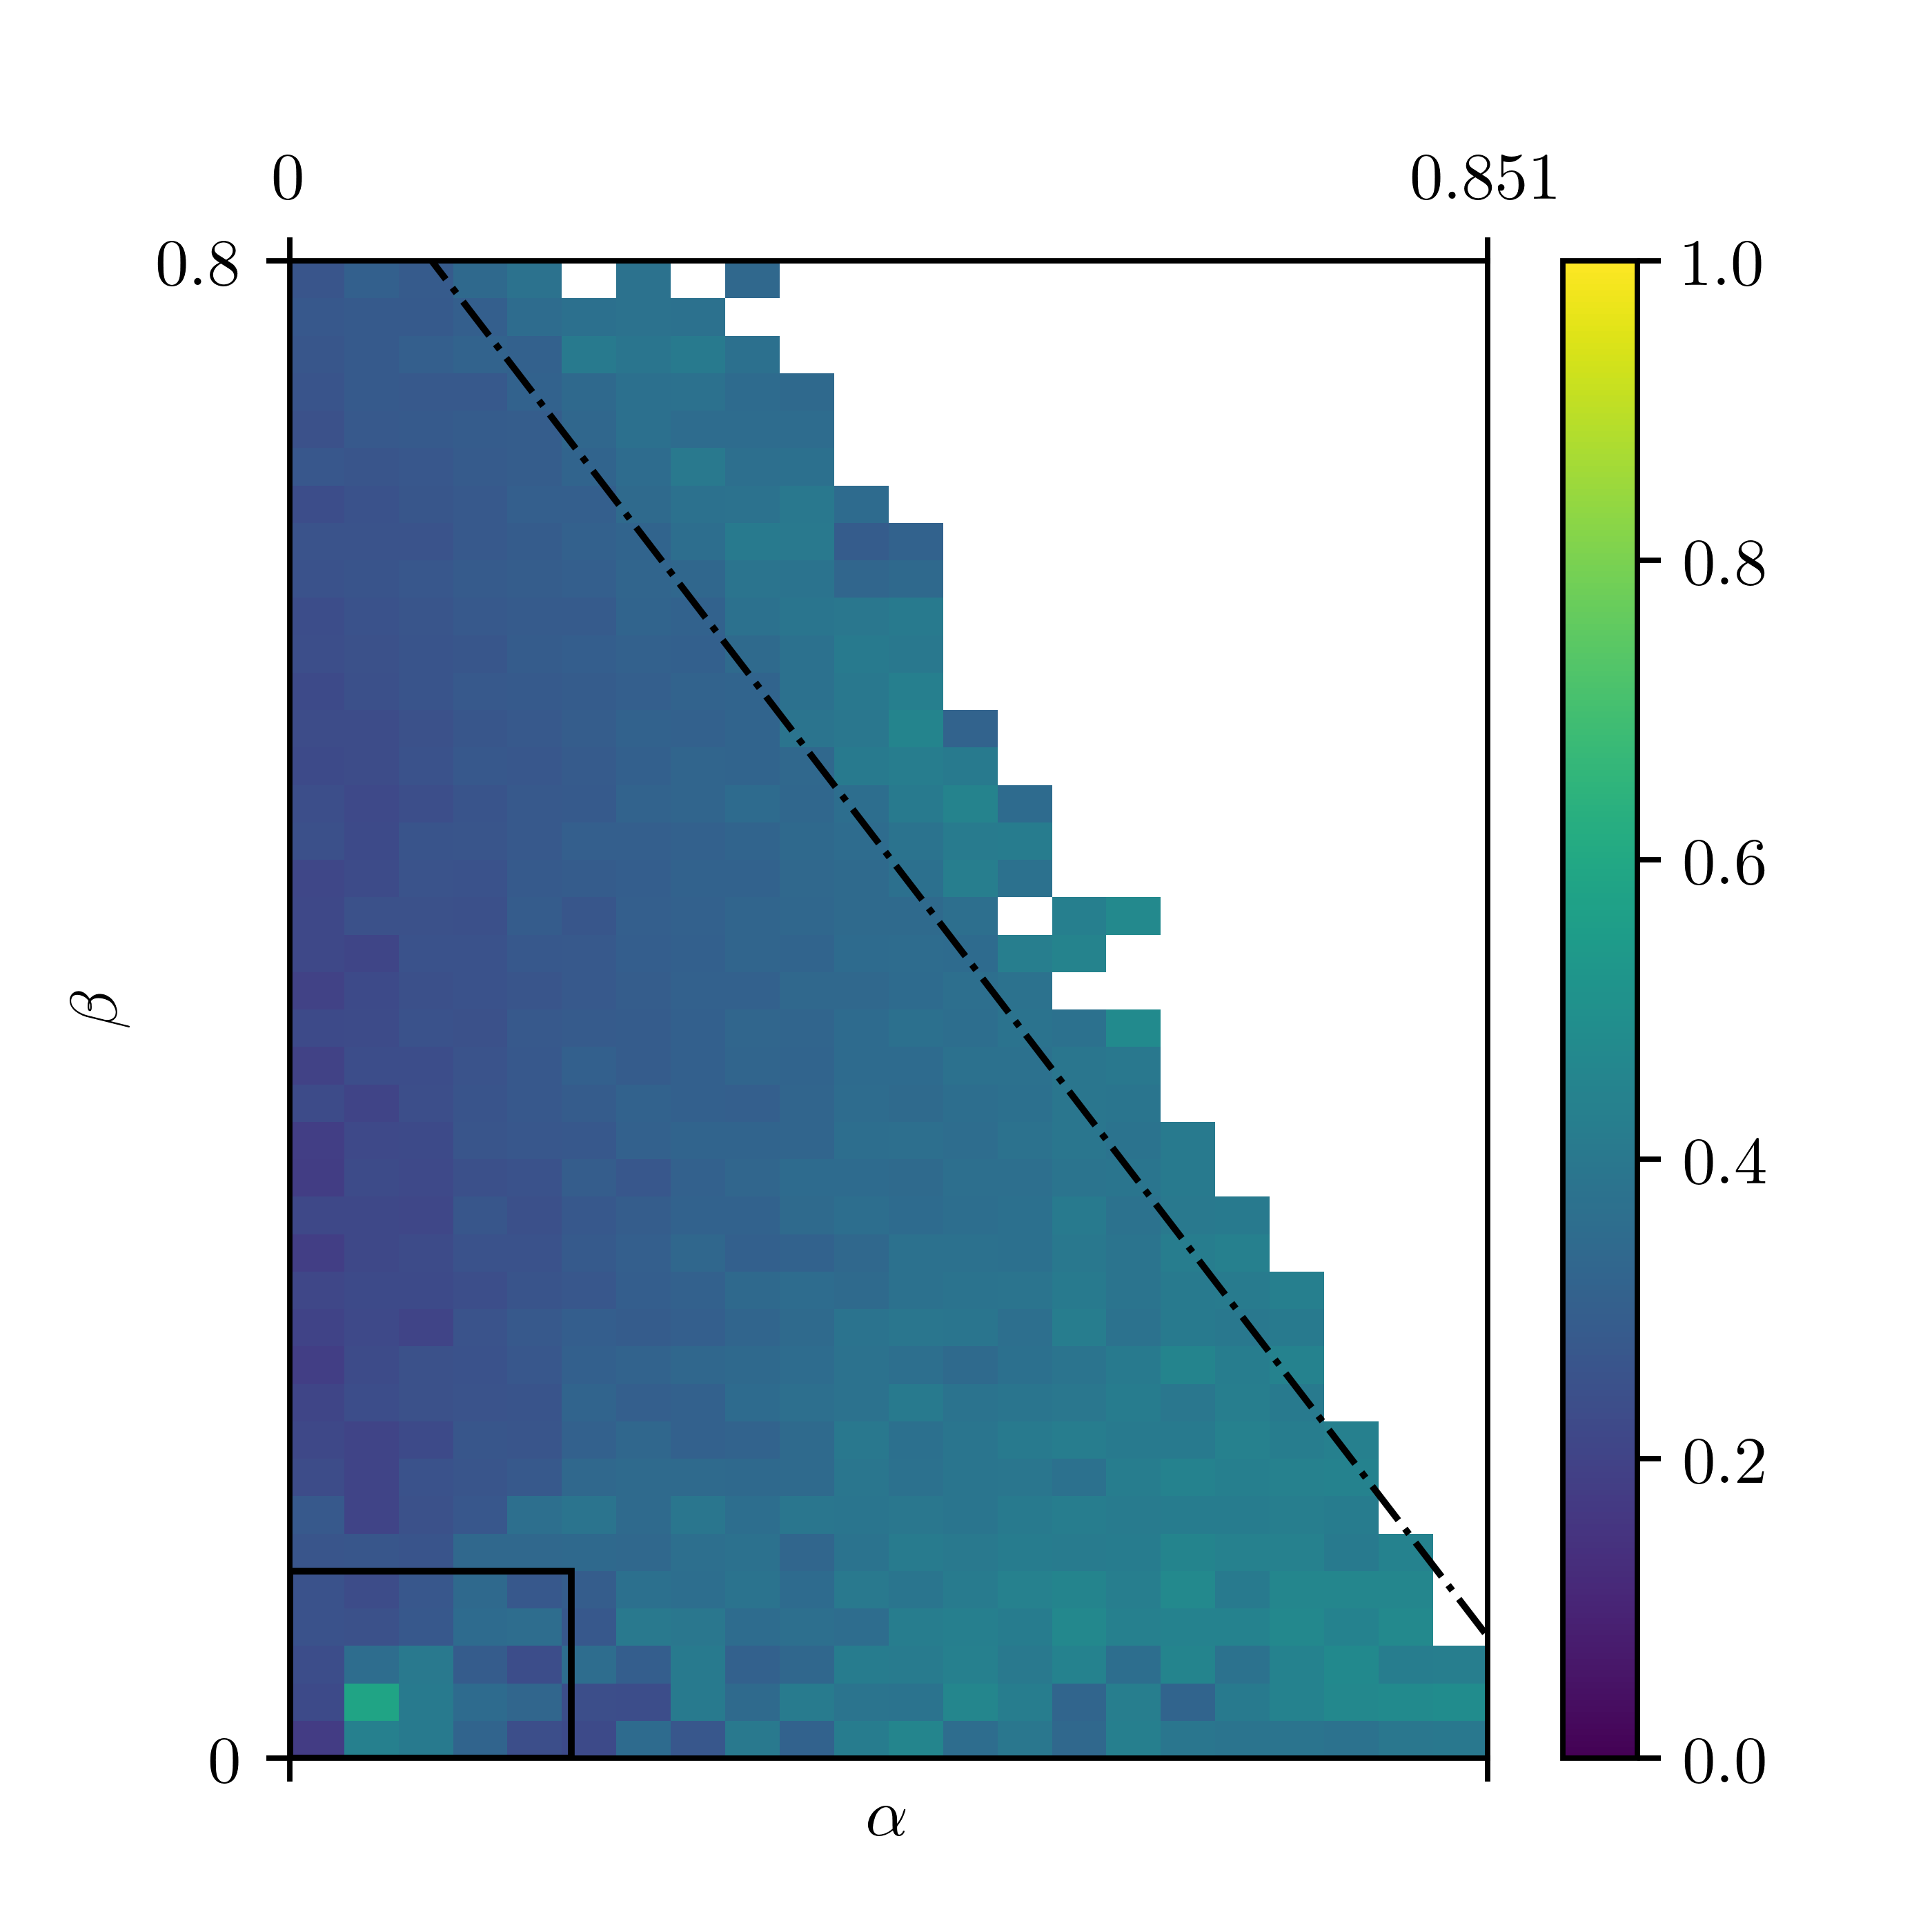
\includegraphics[width=0.5\textwidth]{figure/aphysical_chimera}
    \caption[Chimera-like index landscape]{
      The chimera-like landscape of parameter space on $\pqty{\hra, \hrb} \in \pqty{0, 0.9} \times \pqty{0, 0.9}$.
      The aphysical region of the model is shown in white.
    }
    \label{fig:aphysical_chimera}
  \end{figure}

\end{frame}

\begin{frame}
  \frametitle{That Highly Chimeric Patch}
  \begin{figure}[ht]
    \centering
    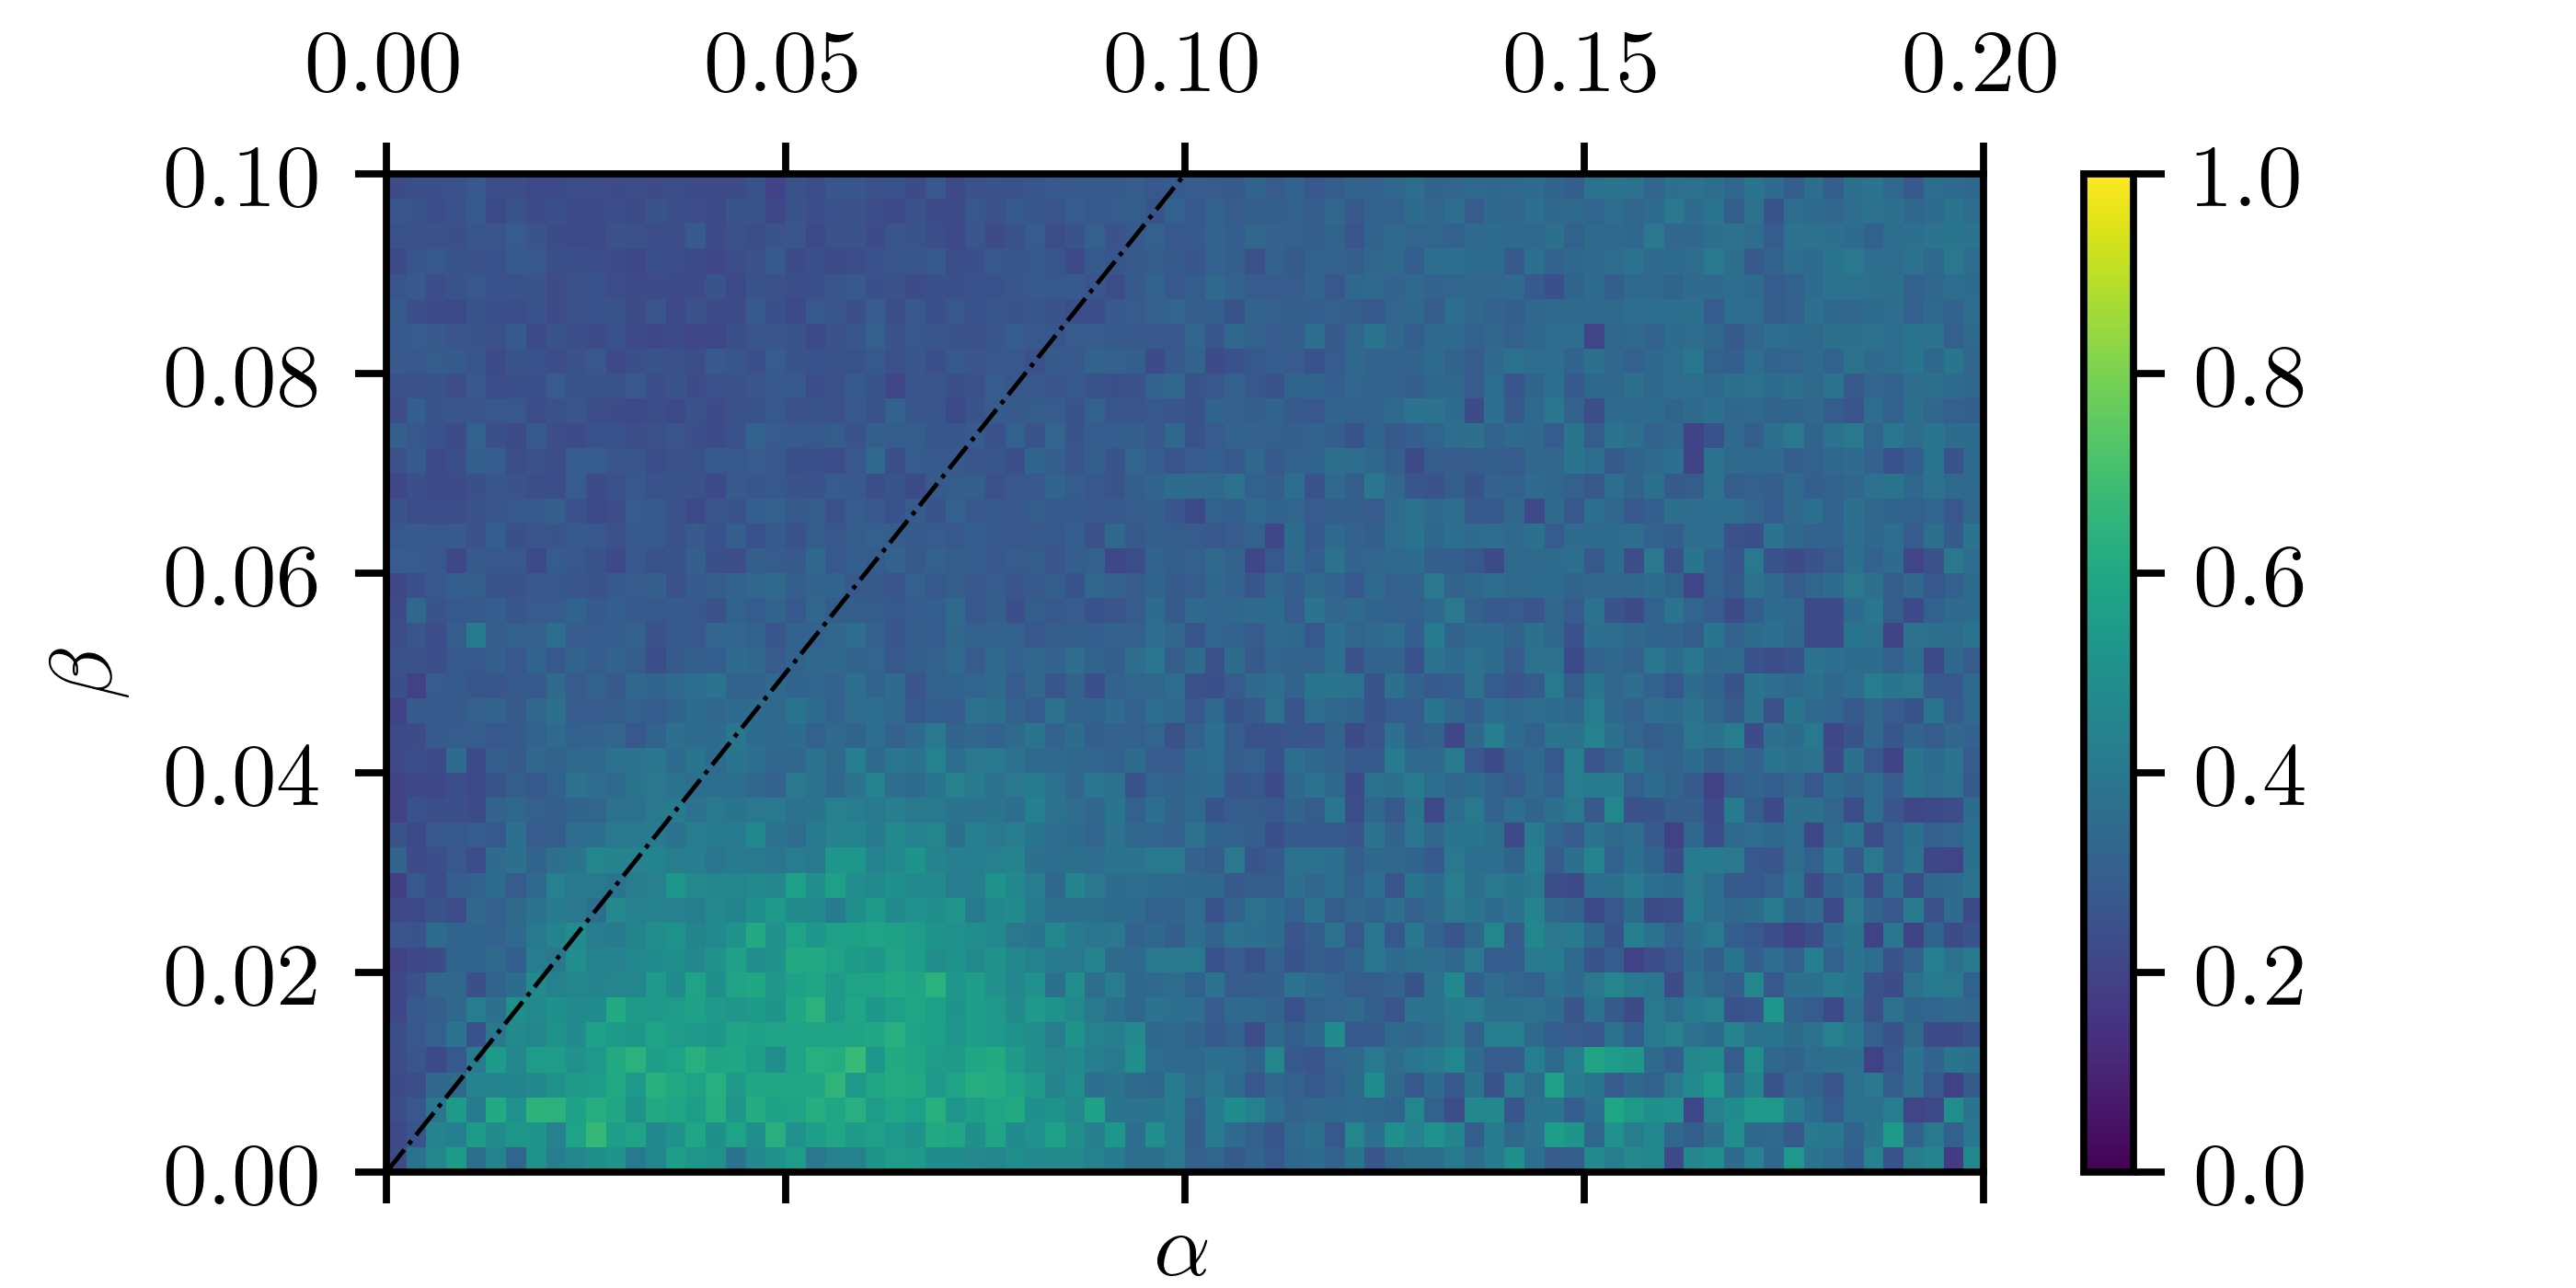
\includegraphics{figure/zoom_chimera}
    \caption[Zoomed landscape]{The chimera index of runs with $(\hra, \hrb) \in (0, 0.2) \times (0, 0.1)$.
      As before, the chimera-like index is normalized to $\frac{1}{7}$.
      The dashed line shows $\beta = \alpha$.
    }
    \label{fig:zoom_chimera}

  \end{figure}

\end{frame}

\begin{frame}
  \frametitle{Yes, It's Real}
  \begin{figure}[ht]
    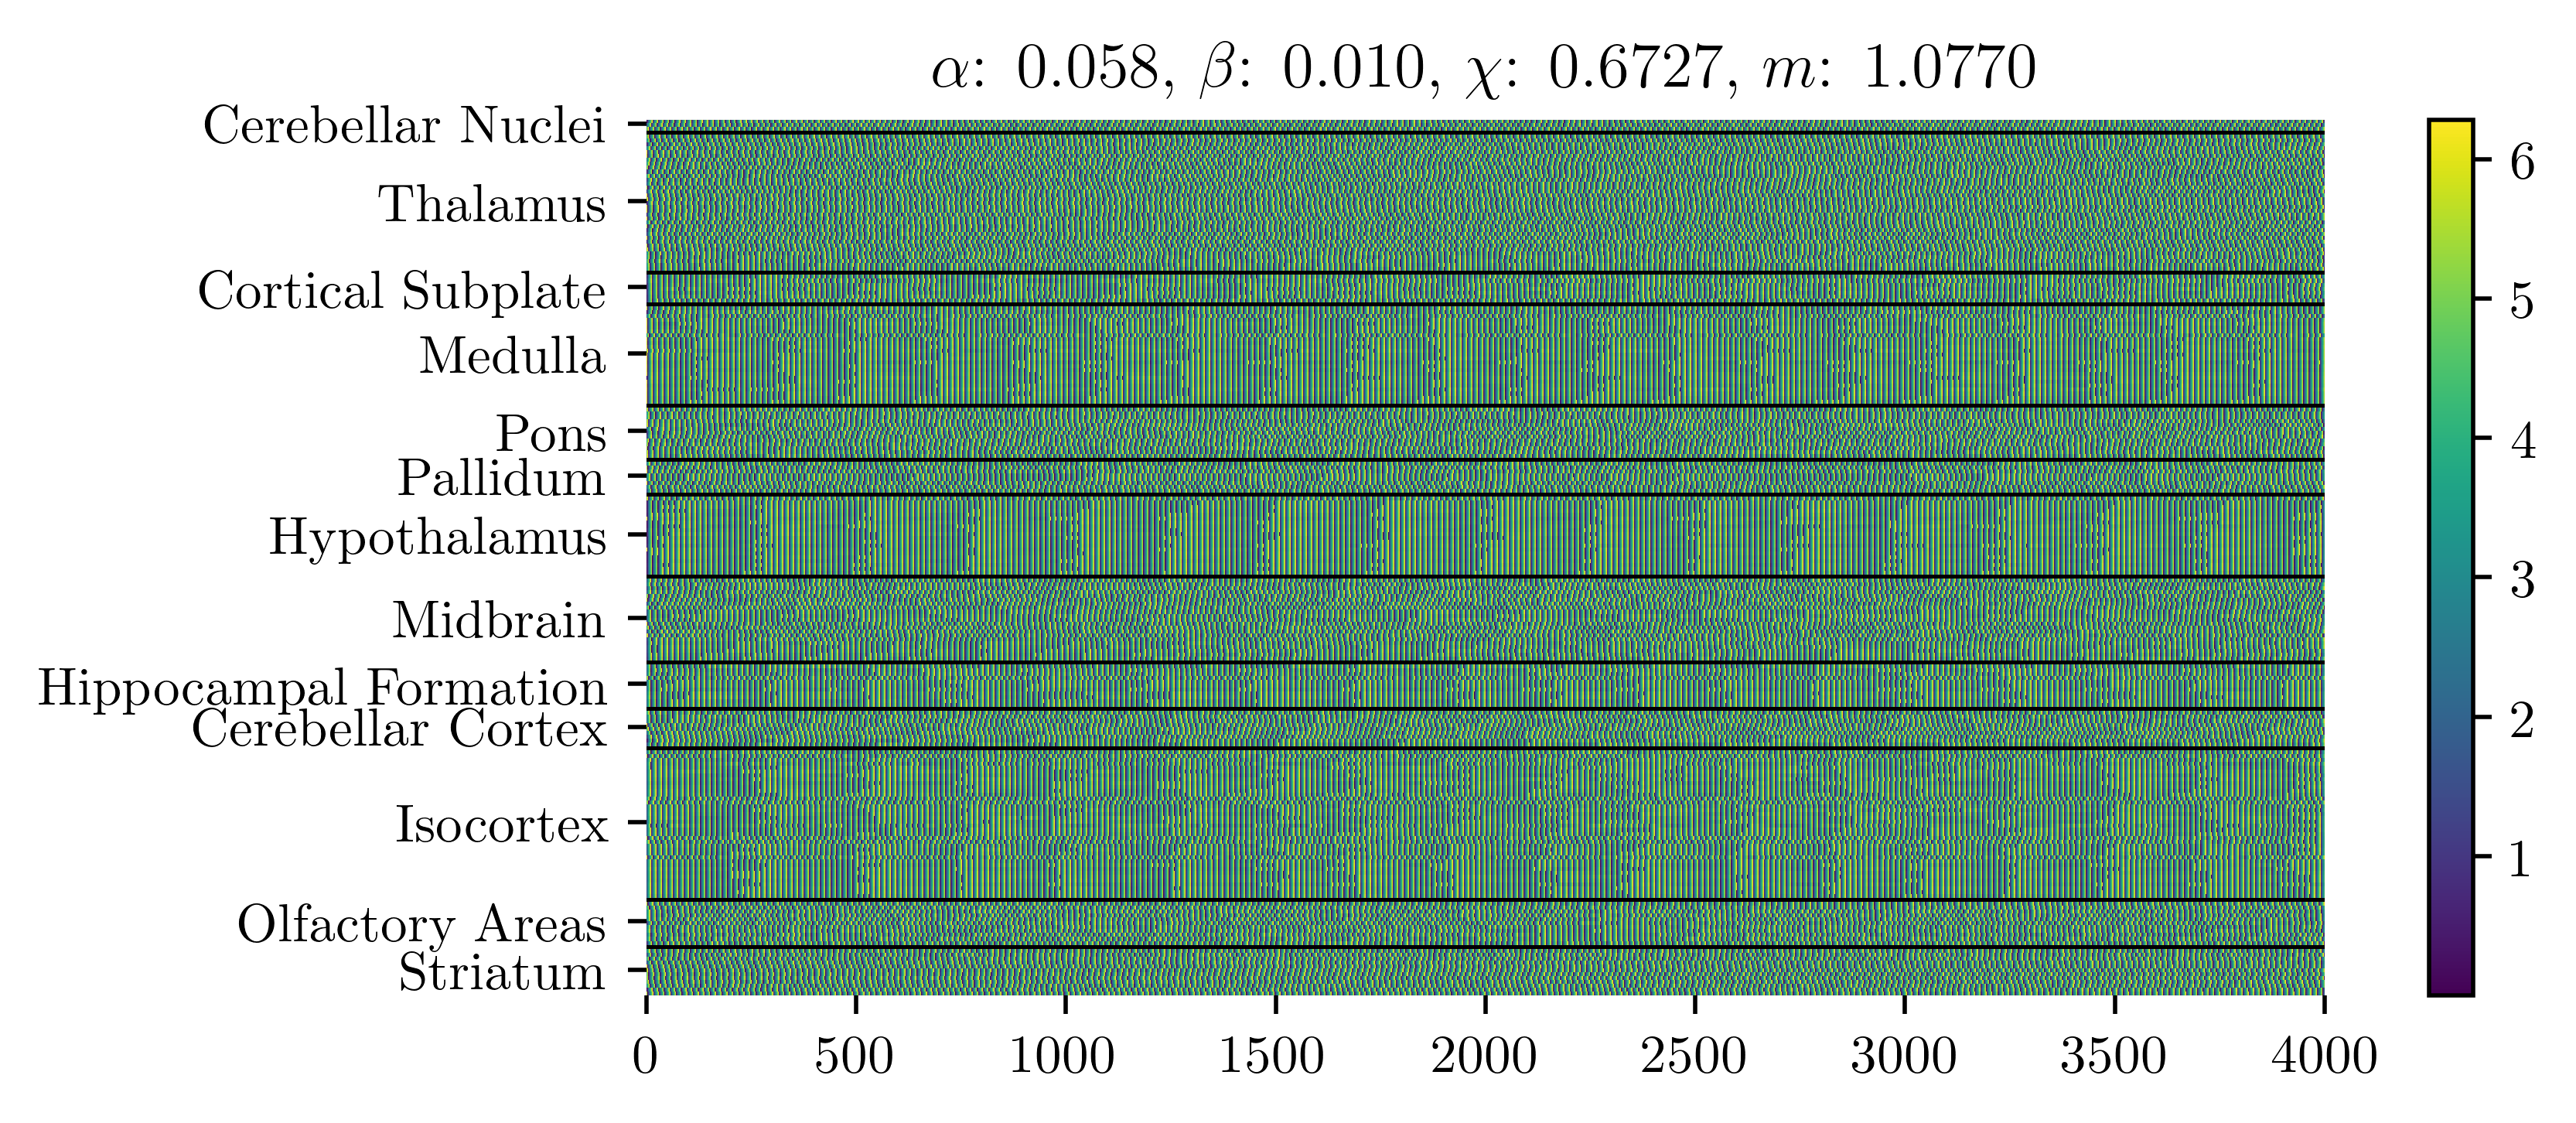
\includegraphics[width=\textwidth]{figure/overhead-0_058-0_010}
    \caption[Highly chimeric simulation]{
      A run of the Hindmarsh-Rose simulation in the chimeric island.
      Synchronization is most consistently evident in the medulla, the hypothalamus, and the isocortex.
    }
    \label{fig:overhead_058_010}
  \end{figure}

\end{frame}
\begin{frame}
  \frametitle{Another Viewpoint}
  \centering
  \movie[showcontrols,loop,width=0.7\textwidth,height=0.7\textwidth,autostart]{An animation of the phase of the simulation.}{figure/animation.mov}
\end{frame}

\begin{frame}[allowframebreaks]
  \frametitle{References}
  \tiny \printbibliography
\end{frame}

\end{document}

%%% Local Variables:
%%% mode: latex
%%% TeX-master: t
%%% End:
